\section{Distributing the Image Reconstruction}\label{distribution}
Distributing the whole image reconstruction. So far, only parts were distributed. First time that end to end, everything gets distributed.

OpenMPI

Gridding and Devonvolution

\subsection{Distributed Gridder: The IDG algorithm}\label{distribution:idg}
Veeneboer et al\cite{veenboer2017image} developed the Image Domain Gridder. It uses Subgrids and solves each subgrid seperately.
It is in the image domain, because it can do Radio Interferometer specific corrections efficiently. Furthermore, it leads to a structure which is primed for GPU processing.
We use this algorithm to distribute the gridding.

W-Projection, Spheroidal are convolutions in the Fourier space.

The figure \ref{distribution:idg:system} shows the different parts of the image domain algorithm.

\begin{figure}[h]
	\centering
	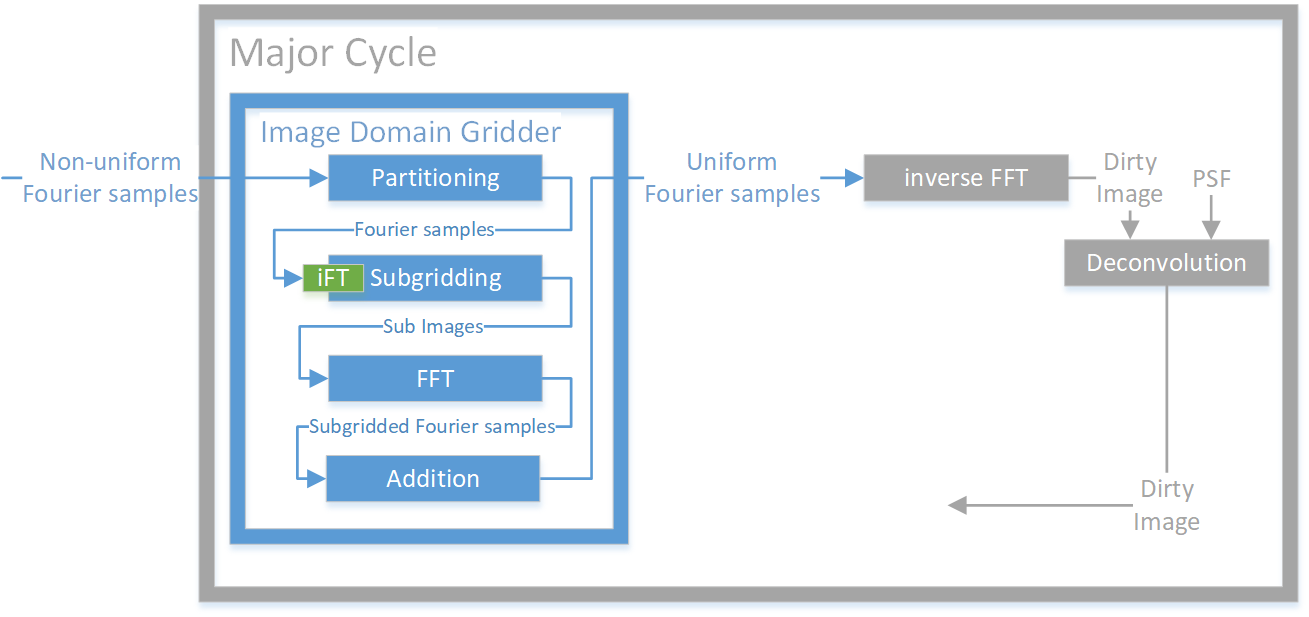
\includegraphics[width=0.80\linewidth]{./chapters/03.distribution/idg/major-minor-idg.png}
	\caption{Image Domain Gridder in the Major Cycle Architecture}
	\label{distribution:idg:system}
\end{figure}

Algorithm
\begin{figure}[h]
	\centering
	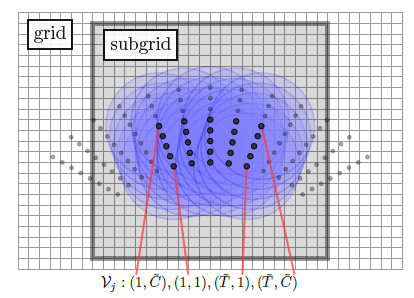
\includegraphics[width=0.40\linewidth]{./chapters/03.distribution/idg/subgrid.png}
	\caption{Subgrid}
	\label{distribution:idg:subgrid}
\end{figure}

\begin{figure}[h]
	\centering
	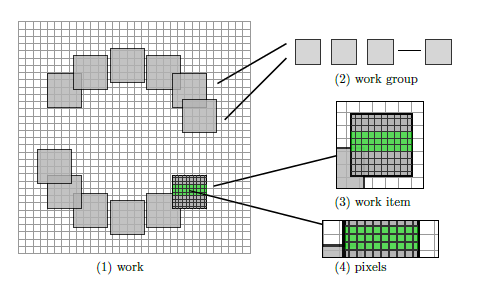
\includegraphics[width=0.40\linewidth]{./chapters/03.distribution/idg/paralellization.png}
	\caption{parallel}
	\label{distribution:idg:parallel}
\end{figure}

\begin{figure}[h]
	\centering
	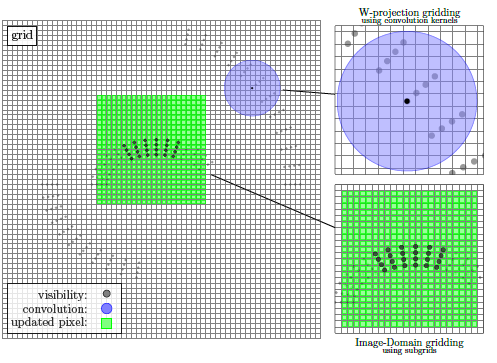
\includegraphics[width=0.40\linewidth]{./chapters/03.distribution/idg/idg0.png}
	\caption{Image Domain Gridder in the Major Cycle Architecture}
	\label{distribution:idg:idg0}
\end{figure}



\subsection{Distributed Deconvolution: Coordinate Descent}

